\chapter{Results and evaluation}
\label{ch:evaluation}

\section{Experiments}

\subsection{Weather and load schedules}
\label{sec:evaluation:schedules}

The weather prediction and user load schedules used for simulations were provided by the Clean Energy Regulator.
The datasets were originally intended for the evaluation (in simulation) of domestic solar hot water systems.
Data provided includes ambient temperature, direct and indirect insolation, cloud coverage, and a load schedule specified in terms of energy drawn.

To produce a more interesting control problem, the load data was modified to include a more realistic scenario where the house is empty during most of the day.
The resulting simulation conditions are shown together in \autoref{fig:cer-data} for two days at the start of June, when my simulations took place.
June was chosen because the control problem is interesting in winter, whereas in summer the sun provides plentiful heat to keep the tank hot with minimal boosting.

\begin{figure}
   \centering
   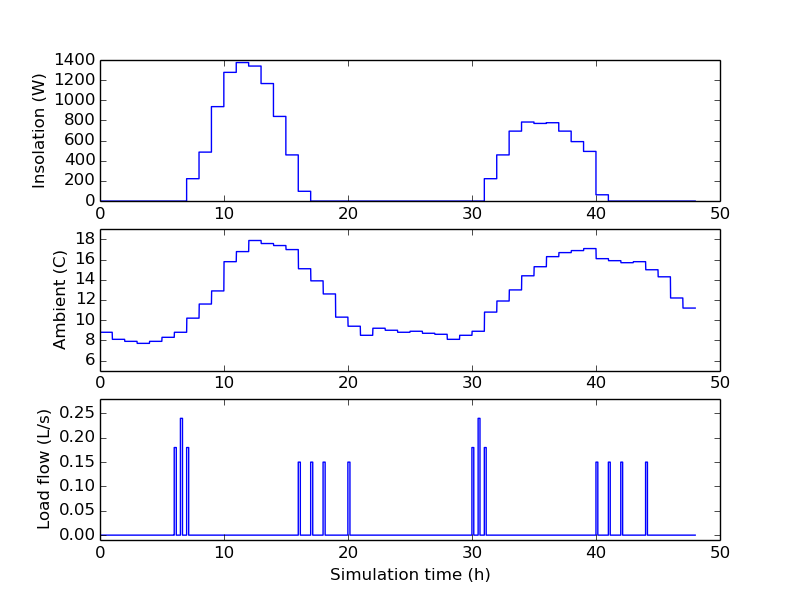
\includegraphics[width=10cm]{images/cer-data}
   \caption{Two days of simulated weather and load conditions}
   \label{fig:cer-data}
\end{figure}

\subsection{Metrics}

The controller's performance was quantified according to three metrics:

\begin{description}
   \item[Satisfaction]
      The user's satisfaction was measured by accumulating the total amounts of time when water was flowing to the user and was at least 50 degrees, and when water was flowing and was less than 50 degrees.
      This number was chosen based on guidelines for domestic water use from Sustainability Victoria~\cite{LSTS}.

   \item[Energy use]
      The total energy use of the controller is integrated across each experiment run.
      This provides an obvious way to compare the strategies of each controller based on how much power they consume to achieve the level of comfort measured by the first metric.
      Note that energy bill is assumed to be implicit in this metric, as this thesis does not take into account the effects of a varying energy price.

   \item[Solar contribution]
      The `solar contribution' refers to the amount of energy gained from sunlight relative to the total amount of energy put into the hot water tank.
      This is a relevant metric as it permits the examination of how effectively the solar resource was exploited.
      However, analysis is complicated by the relationship between solar fraction and total energy used by the controller.
      If one controller expends less control power, all else being equal, it will tend to have a higher solar contribution simply because the amount of energy gained from the sun is now greater in comparison.
      However, this metric does take into account the effect of a tank kept too-hot, which will result in the solar pump differential controller never choosing to let water enter the tank, thereby reducing solar contribution.
\end{description}

These metrics were evaluated each minute during the simulation.

\subsection{Experiment specifications}

\subsubsection{Experiment 1. Comparison to thermostat control}

The goal of this experiment is to compare the predictive controller to the baseline thermostat controller.
For each of the two controllers, eight simulations were run.
Each simulation lasted for one week, and weeks were evenly distributed in December, January, June, and July to compare the operation of the controllers in summer and winter.
It is expected that the predictive controller will have a lower energy usage than the baseline thermostat, but most likely at the cost of some user satisfaction.

\subsubsection{Experiment 2. The effect of inaccurate predictions}

To gauge how critical the effect of prediction accuracy is to the controller's performance, an experiment was set up comparing the controller on a week in July with perfect prediction (as is standard in all other experiments) and with an incorrect prediction that overestimated how much solar energy would be available.
\Autoref{fig:insolation-error} shows two days from the two profiles used for simulation and prediction.
The predicted profile is identical each day, and overpredicts the amount of insolation.
The true profile is a standard July week.

\begin{figure}
   \centering
   \begin{adjustwidth}{-2cm}{-2cm}
   \begin{subfigure}[b]{0.65\textwidth}
      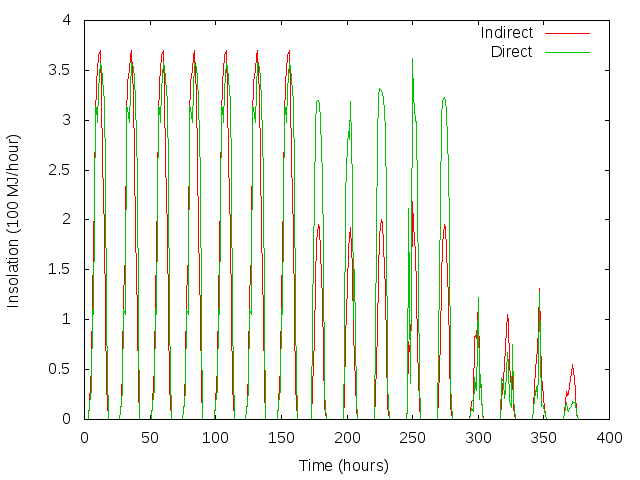
\includegraphics[width=\textwidth]{images/insolation-prediction}
      \caption{Insolation prediction}
      \label{fig:insolation-error-p}
   \end{subfigure}
   ~ %add desired spacing between images, e. g. ~, \quad, \qquad, \hfill etc.
   \begin{subfigure}[b]{0.65\textwidth}
      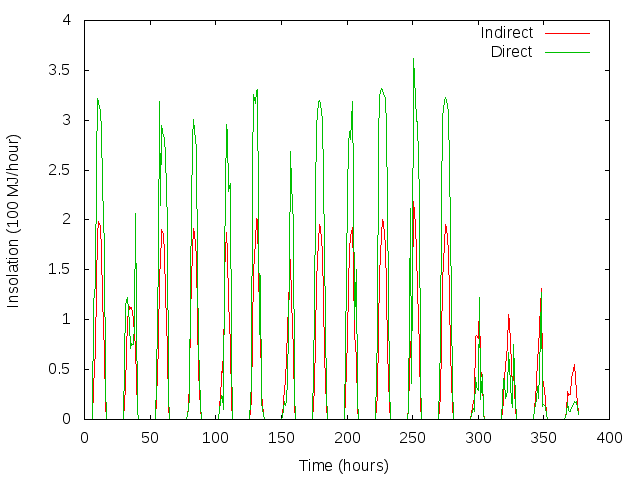
\includegraphics[width=\textwidth]{images/insolation-actual}
      \caption{Actual insolation}
      \label{fig:insolation-error-t}
   \end{subfigure}
   \end{adjustwidth}
   \caption{Insolation profiles for experiment 2}
   \label{fig:insolation-error}
\end{figure}

\subsubsection{Experiment 3. The effect of the control weight}
\label{experiment3}

The controller was designed with a tuning parameter $\rho$ (see \autoref{eq:controller-problem}).
A series of simulations was run with identical conditions except for this parameter.
Eight values were used, arranged linearly from $1\e{-9}$ to $1\e{-5}$.
This was determined to be the range over which the controller varied from maximum satisfaction, keeping the tank very warm most of the time, down to roughly 85\% satisfaction, and only heating the tank immediately before a period of use.

Note that other experiments were conducted with $\rho = 1$.
This provides slightly less comfort and energy usage than the smallest value used in this experiment, and was found to be a good match for thermostat control.

\subsubsection{Experiment 4. The effect of the prediction horizon}

For completeness, it is desirable to determine what effect, if any, the length of the prediction horizon has on the controller's behaviour.
To determine this, a week-long experiment was run five times with controller prediction horizons varying from 4 to 12 hours.
Longer timeframes were not investigated, based on the results achieved from these simulations.

\subsection{Results}

\subsubsection{Experiment 1. Comparison to thermostat control}

\Autoref{fig:comparison} shows the results across all three metrics measured in the sixteen simulations performed for experiment 1.
The source data of this chart is listed in \autoref{tab:comparison}.
Each set of three metrics is a single simulation.
Two simulations were performed in each month for each controller.
All results for MPC are in the left half of the chart, whereas thermostat results are on the right.

\begin{figure}
   \centering
   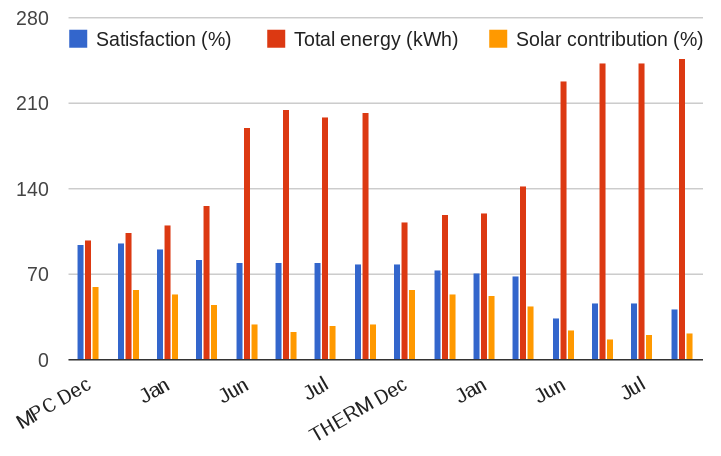
\includegraphics[width=\textwidth]{images/comparison}
   \caption{Comparison of predictive and thermostat control}
   \label{fig:comparison}
\end{figure}

Broad trends are visible.
Predictably, the controllers both use more energy in winter, and have lower user satisfaction and solar fraction.
Also notice that the predictive controller has higher satisfaction and lower power usage in corresponding experiments.
However, this effect appears only marginal.

As noted in \autoref{experiment3}, the value $\rho=1$ was used for these simulations.
This assigned a fairly hefty penalty to use of the control signal, and caused most days to follow a heating regimen similar to that of \autoref{fig:mpc-comparison}, which shows a single day from the first June simulation.
The controller fires just before the two main periods of water use during the day, with some use during the middle of the day to counteract the effects of ambient cooling.
Contrast this to the profile in \autoref{fig:thermostat-comparison}, where the main periods of heating are just \emph{after} peak load times.

Also of interest is the smoother profile shown by the MPC controller.
This is a result of the rapid (10 minute period) PWM used to interpret the MPC's continuous control inputs.
The thermostat, on the other hand, can only respond when the temperature falls below its deadband, and causes the sawtooth seen in the middle of the day.

\begin{figure}
   \centering
   \begin{subfigure}[b]{0.85\textwidth}
      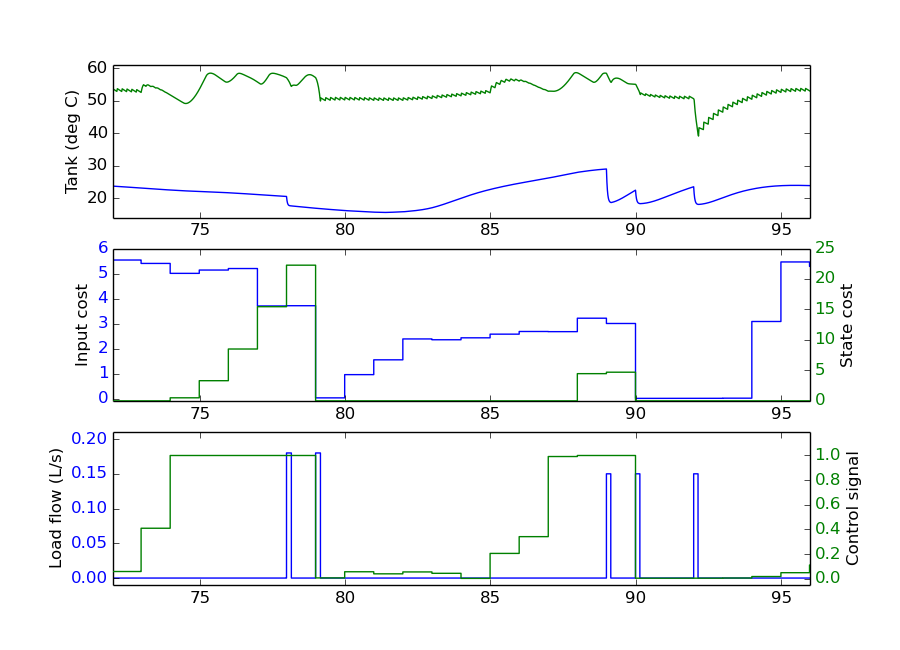
\includegraphics[width=\textwidth]{results/mpc-comparison-6-1}
      \caption{MPC heating action}
      \label{fig:mpc-comparison}
   \end{subfigure}
   \\ %add desired spacing between images, e. g. ~, \quad, \qquad, \hfill etc.
   \begin{subfigure}[b]{0.85\textwidth}
      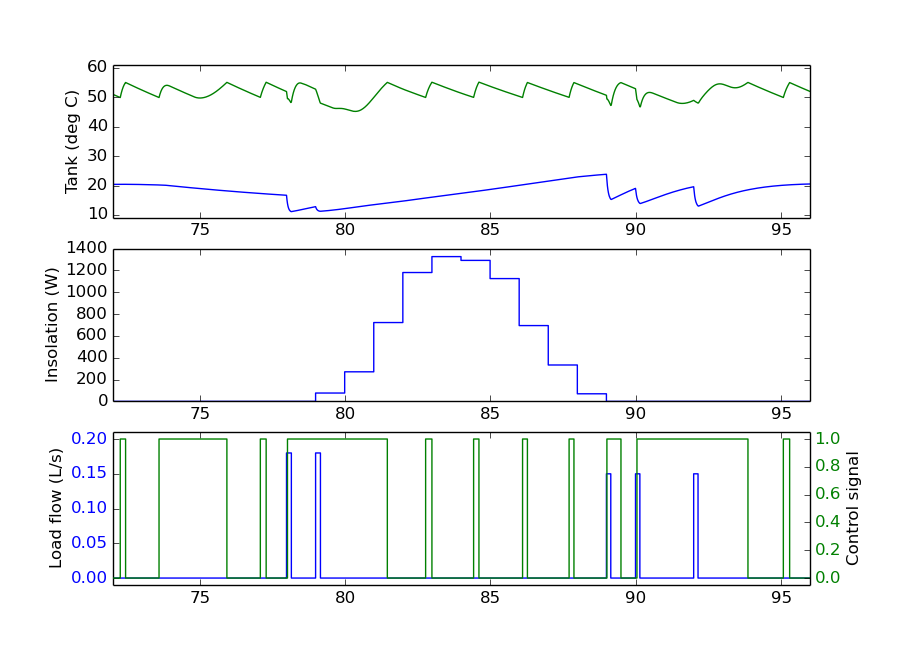
\includegraphics[width=\textwidth]{results/thermostat-comparison-6-1}
      \caption{Thermostat heating action}
      \label{fig:thermostat-comparison}
   \end{subfigure}
   \caption{Examples of heating profiles of two controllers}
   \label{fig:profile-comparison}
\end{figure}

\subsubsection{Experiment 2. The effect of inaccurate predictions}

The effect of erroneous solar predictions appeared to be minimal.
An example of the predictions affecting the controller over a single day is shown in \autoref{fig:mpc-error}.
The pink lines in the temperature plot show, at each hour, the predicted future average temperatures the controller expects.
Over midday, when insolation would have the greatest effect, a large pink crest indicates the controller's optimistic expectation of large solar gains.
However, this still only resulted in a modest decrease in energy use by the controller, and a small violation of the user's comfort.

\begin{figure}
   \centering
   \includegraphics[width=12cm]{results/mpc-prediction-error}
   \caption{A day in the life of a controller with bad predictions}
   \label{fig:mpc-error}
\end{figure}

\subsubsection{Experiment 3. The effect of the control weight}

The parameter $\rho$ caused predictable changes in the control response.
Higher values imposed a more severe penalty on using any control input, while lower values allowed the controller to take any means necessary to avoid accruing penalties due to the comfort requirement.
\Autoref{fig:mpc-rho} illustrates this with two control profiles from this experiment.

\Autoref{fig:rho-graphs} shows the trends in each metric as functions of $\rho$.
It makes clear the downward trend in comfort and energy usage as values of $\rho$ increase.
The data which produced this graph is listed in \autoref{tab:rho}.

\begin{figure}
   \centering
   \begin{subfigure}[b]{0.85\textwidth}
      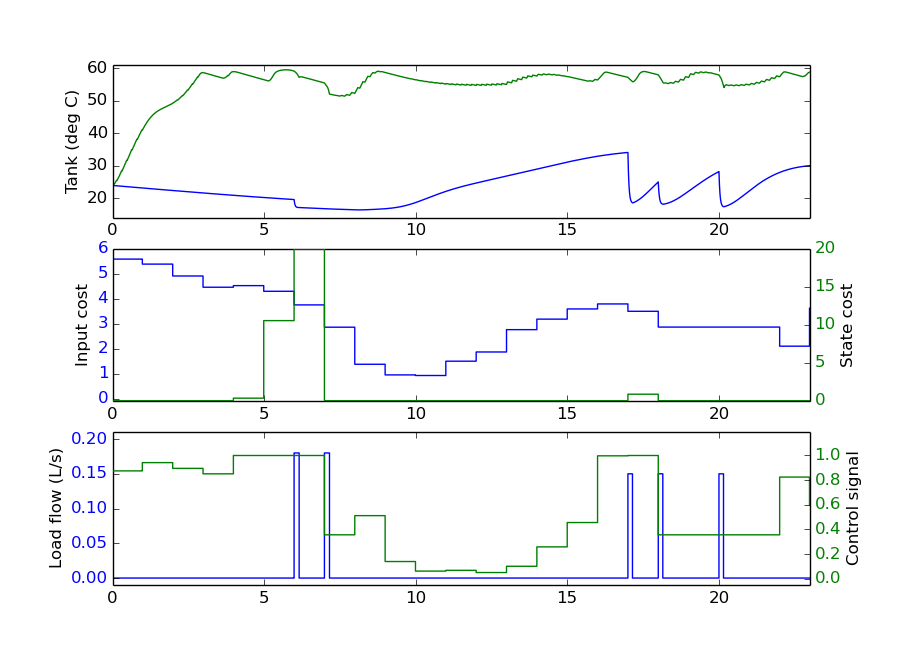
\includegraphics[width=\textwidth]{results/mpc-rho-19}
      \caption{With $\rho = 1\e{-9}$}
      \label{fig:mpc-rho-small}
   \end{subfigure}
   \\
   \begin{subfigure}[b]{0.85\textwidth}
      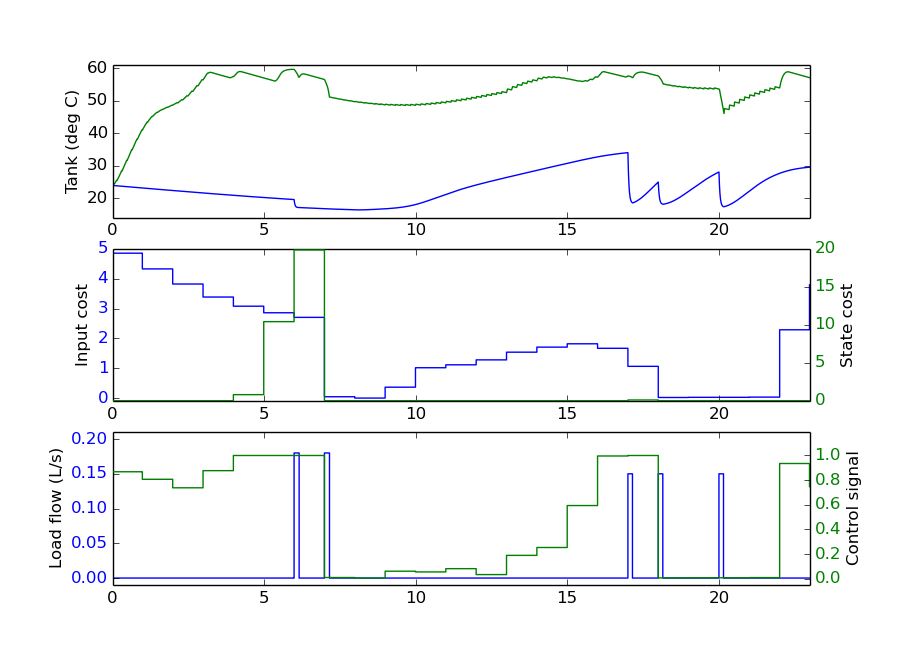
\includegraphics[width=\textwidth]{results/mpc-rho-57}
      \caption{With $\rho = 5\e{-7}$}
      \label{fig:mpc-rho-larger}
   \end{subfigure}
   \caption{Simulations with two values of the tuning parameter $\rho$}
   \label{fig:mpc-rho}
\end{figure}

\begin{figure}
   \centering
   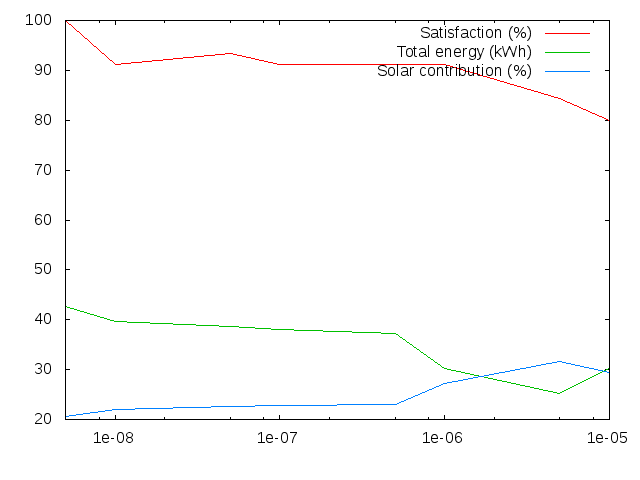
\includegraphics[width=10cm]{images/rho-graphs}
   \caption{Effects of $\rho$ on the three metrics}
   \label{fig:rho-graphs}
\end{figure}

\subsubsection{Experiment 4. The effect of the prediction horizon}

The effect of the planning horizon appeared to be minimal.
Above a horizon of four hours, the controller could not take advantage of increased prescience.
The results are presented in \autoref{tab:H}, but are not very interesting.

\section{Discussion}

\subsection{Interpretation}

The discussion in this section must be prefaced with a word of caution: the simulations presented should be taken anecdotally, rather than as statistically significant.
The reader must also bear in mind that they were conducted with a highly unrealistic scenario, both in terms of the load pattern, and the controller's ability to predict future disturbances.

\subsubsection{Performance}

The controller did not achieve the significant gains seen for MPC in other research.
At most, it decreased energy usage by around 10\%, and increased user satisfaction by the same amount.
These results are not trivial, but do not approach the 30\% that \authors{Halvaard12}, for example, were able to achieve.
It also remains to be seen whether this performance benefit would apply to real systems.

However, the fundamental difference of MPC has been made clear by comparison to the thermostat controller.
The predictive controller consistently heats the tank \emph{in advance} of a large period of load, whereas the thermostat reheats the tank \emph{in response} to one.
This is a fundamental difference that demonstrates the controller's utility.

\subsubsection{Tuning}

An interesting result from experiment 3 was the process of tuning $\rho$.
While MPC is said to be `intuitive' in its tuning --- and this is largely true --- it was at first difficult to find values of $\rho$ that had the desired effect.
There also appears to be a large inexplicable plateau between the values of $1\e{-5}$ and 1, where the controller behaves largely the same no matter the tuning parameter.
For larger values than 1, the controller will start to become conservative very quickly, hardly expending any effort at all with $\rho=10$.

The process of finding the values that would display an interesting portion of the metrics curves shown in \autoref{fig:rho-graphs} took more time than running those simulations with the correct numbers once they were found.
This has interesting implications for the design process.
How should parameters like $\rho$ be tuned by the designers?
And how, if at all, should they be exposed to user tuning?

The effect of $\rho$ has an obvious and intuitive meaning as a balance between comfort and control expense.
But the actual effects on the user of a certain change in $\rho$ may not be simple, even when measured as a statistic like the satisfaction metric presented here.

The results of experiment 4, tuning the control horizon, appear to agree with the findings of \textcite{Halvgaard12}.
They noted that increasing the lookahead further than 24 hours did not gain them anything.
It appears that 24 hours is a `natural' length of time for their controller to work with, given the physical dimensions of their tank, actuators, and disturbances --- such as cheaper energy prices occurring nightly.
I hazard to suggest that the `natural' period of the control problem examined in this thesis is shorter due to the dynamics of the smaller tank, which is mostly governed not by a nightly energy price, but by the user's load schedule.

\subsection{Future work}

Evidently this controller still has its limitations, as does the evaluation presented in this thesis.
The most obvious work that needs to be done is greater experimental coverage of the design space, both to test the controller's robustness and to begin to make statistically valid conclusions.
Heavier and less regular load profiles should be used, and more combinations of controller variables should be tested in combination (a 2D gridded approach, rather than the several 1D experiments presented here).

Due to time constraints, this thesis never explored more complex control models.
A simple extension would be to add a two-zone model of the controller, where the temperatures of the top and bottom of the tank were treated independently.
This becomes interesting considering that the auxiliary heater only heats the top half of the tank.
It may allow the controller to make more informed decisions about how much of the tank it should heat.

And finally, the option of nonlinear control remains.
The simulation model presented was bilinear, and with certain simplifying assumptions together with the removal of the internal controllers, could be made smooth.
It would then be suitable for modelling and control with software such as ACADO.
It would be necessary in this case for the controller to take responsibility for all pumps and valves in the system, to remove all non-smoothness from the model itself.
This would present even more opportunities for the controller to intelligently manage the system.

Finally, immediate future work must include improvements to the tank model itself.
This model still leaves some important factors unaccounted for, such as pressure release valves on the tank and collector.
Validation against a real system would help to tune the constants involved, which for this thesis were simply set to plausible values based on qualitative descriptions of how hot water systems commonly behave --- or were approximated from values found in datasheets or other studies.

\section{Conclusion}

This thesis has presented a successful model-predictive control algorithm for use on domestic solar water systems.
It was shown to be a viable competitor to the thermostat controller in simulations, having slightly reduced energy usage and slightly increased user satisfaction in both winter and summer months.

Much work remains to be done, but this appears to be a promising start.
